
\documentclass[a4paper,12pt]{article}

% Packages for formatting and functionality

\usepackage[utf8]{inputenc} % Input encoding
\usepackage[T1]{fontenc}   % Font encoding
\usepackage{amsmath, amssymb} % Math symbols
\usepackage{graphicx}      % Including images
\usepackage{hyperref}      % Hyperlinks
\usepackage{geometry}      % Page layout
\usepackage{titlesec}      % Section formatting
\usepackage{booktabs}      % Tables
\usepackage{tabu}          % tables
\usepackage[labelfont=bf, skip=5pt, font=small]{caption} %format tabu captions
\usepackage{subcaption}    %typeset captions for sub-tables/figures
\usepackage{tikz}          %for adding images (since no screenshots)
\usetikzlibrary{shapes.geometric, arrows.meta, positioning,backgrounds}
\usepackage{longtable}     % Long tables
\usepackage{xcolor}        % Text colors
\usepackage{float}         % Positioning of figures and tables
\geometry{margin=1in}      % Margins
\usepackage{changepage}    %modify single-page layouts
\usepackage{siunitx}       %properly typeset Units
\usepackage{pgfplots} %Embedding GNUPlots
\pgfplotsset{compat=1.18} 


% Hyperlink setup
\hypersetup{
    colorlinks=true,
    linkcolor=blue,
    filecolor=magenta,  
    urlcolor=cyan,
    pdftitle={Function Generator Report},
    pdfpagemode=FullScreen,
}


\begin{document}

\begin{center}
    {\Huge\textbf{ELP305 P1 Report}\par}
    \vspace{0.15cm}
    {\Large Function Generator --- Requirements\par}    
    \vspace{0.1cm}
    \large \textcolor{darkgray}{Thursday Tribe}
\end{center}

\hspace*{-1in}  
\rule{1.2\linewidth}{0.4pt}

\begin{figure}[H]
\hspace*{-0.72in}  
\begin{minipage}[t]{0.7\textwidth}
    \centering
    
\tikzset{
    default/.style={fill=blue!5, draw=black!50, line width=1pt, text width=2.6cm, align=center, rounded corners, minimum height=1.5cm},
    current/.style={fill=blue!30, draw=blue, line width=2pt, text width=2.8cm, align=center, rounded corners, minimum height=1.5cm, font=\bfseries},
    arrow/.style={-{Latex[round]}, line width=1pt, draw=black!50}
}


\begin{tikzpicture}[node distance=2.5cm and 1cm]

% Nodes
\node[current] (R) {Requirements};
\node[default, right=of R] (S) {Specifications};
\node[default, right=of S] (D) {$N \times$ Design-Cycles};
\node[default, right=of D] (M) {$N \times$ MajorRel};
\node[default, above right=1cm and 1cm of M] (C) {Closure};
\node[default, below right=1cm and 1cm of M] (Min) {$N \times$ MinorRel};

% Arrows
\draw[arrow] (R) -- (S);
\draw[arrow] (S) -- (D);
\draw[arrow] (D) -- (M);
\draw[arrow] (M) -- (C);
\draw[arrow] (M) -- (Min);
\draw[arrow, <->] (Min) to[bend left=30] (M);

\end{tikzpicture}

 
    \label{fig:front_cover}
\end{minipage}
\end{figure}

% \vspace{-0.4cm}
% \hspace*{-1in}  
% \rule{1.2\linewidth}{0.4pt}



\tableofcontents

\newpage
\section{List of Tables}
\listoftables

\newpage
\section{List of Figures}
\listoffigures
% \addcontentsline{toc}{section}{List of Tables}

% Table captions
% \begin{table}[H]
%     \label{tab:coordinators}
% \end{table}

% \begin{longtable}{l}
%     \label{tab:documentation}
% \end{longtable}

% \begin{longtable}{l}
%     \label{tab:electronics}
% \end{longtable}

% \begin{longtable}{l}
%     \label{tab:mechanical}
% \end{longtable}

% \begin{longtable}{l}
%     \caption{Software Team Members}
%     \label{tab:software}
% \end{longtable}

\newpage
\section{Abbreviations}
\begin{itemize}

% Technical Terms
\item \textbf{AD9833:} Programmable Waveform Generator
\item \textbf{BNC:} Bayonet Neill-Concelman
\item \textbf{ESP32:} Espressif Systems Microcontroller
\item \textbf{LCD:} Liquid Crystal Display
\item \textbf{OLED:} Organic Light-Emitting Diode
\item \textbf{PCB:} Printed Circuit Board
\item \textbf{RF:} Radio Frequency
\item \textbf{SNR:} Signal-to-Noise Ratio
\item \textbf{SPI:} Serial Peripheral Interface
\item \textbf{THD:} Total Harmonic Distortion
\item \textbf{USB:} Universal Serial Bus

% Project Management & Organization
\item \textbf{SPOC:} Single Point of Contact
\item \textbf{IF:} Involvement Factor
\item \textbf{TC:} Tribe Coordinator
\item \textbf{DTC:} Deputy Tribe Coordinator

% Measurements & Units
\item \textbf{Hz:} Hertz
\item \textbf{MHz:} Megahertz
\item \textbf{V:} Volt
\item \textbf{mV:} Millivolt
\item \textbf{W:} Watt
\item \textbf{A:} Ampere
\item \textbf{mA:} Milliampere
\item \textbf{dB:} Decibel

% Environmental & Operating Conditions
\item \textbf{RH:} Relative Humidity
\item \textbf{TEMP:} Temperature

% Standards & Protocols
\item \textbf{Type-C:} Universal Serial Bus Type-C
\item \textbf{I²C:} Inter-Integrated Circuit
\item \textbf{UART:} Universal Asynchronous Receiver-Transmitter

% Signal Types & Characteristics
\item \textbf{AC:} Alternating Current
\item \textbf{DC:} Direct Current
\item \textbf{p-p:} Peak-to-Peak
\item \textbf{RMS:} Root Mean Square

% Quality & Testing
\item \textbf{QC:} Quality Control
\item \textbf{QA:} Quality Assurance
\item \textbf{EOL:} End of Life
\item \textbf{MTBF:} Mean Time Between Failures

% Safety & Compliance
\item \textbf{ESD:} Electrostatic Discharge
\item \textbf{EMI:} Electromagnetic Interference
\item \textbf{EMC:} Electromagnetic Compatibility

\end{itemize}

\newpage
\section{Glossary}

\begin{description}
    \item[AD9833] A programmable waveform generator integrated circuit capable of producing sine, triangular, and square waves
    
    \item[BNC Connector] Bayonet Neill-Concelman connector; a type of RF connector commonly used for signal output in test equipment
    
    
    \item[ESP32] A series of low-cost, low-power microcontroller with integrated Wi-Fi and Bluetooth capabilities
    
    
    \item[LCD] Liquid Crystal Display; a flat-panel display technology
    
    
    \item[OLED] Organic Light-Emitting Diode; a display technology offering high contrast and low power consumption
    
    \item[PCB] Printed Circuit Board; a board that mechanically supports and electrically connects electronic components
    
    \item[RF] Radio Frequency; refers to oscillating electromagnetic waves
    
    \item[SNR] Signal-to-Noise Ratio; measure of signal strength relative to background noise
    
    \item[SPI] Serial Peripheral Interface; a synchronous serial communication protocol
    
    
    \item[THD] Total Harmonic Distortion; measurement of waveform distortion, expressed as a percentage
    
    \item[USB Type-C] Universal Serial Bus Type-C; a standard connector for power delivery and data transfer
    
\end{description}

\newpage
\section{Team Members}
\subsection{Coordinators}
% \begin{longtable}[H]
%     \centering 
%     \begin{tabu}{X[c]|X[c]|X[c]|X[c]|X[c]} 
%         \toprule 
%         \textbf{Designation} & \textbf{Name} & \textbf{Entry No} & \textbf{Email} & \textbf{Phone} \\ 
%         \midrule 
%         Tribe Coordinator & Shahid  &  &  &  \\ 
%         \midrule
%         Deputy Tribe Coordinator &  &  &  &  \\ 
%         \bottomrule 
%     \end{tabu} 
%     \label{tab:coordinators}
%     \caption{Coordinators}
% \end{longtable}
\begin{longtable}[c]{|l|l|l|l|l|l|l|}
\hline
\textbf{Designation} & \textbf{Name} & \textbf{Entry No} & \textbf{Email} & \textbf{Phone} & \textbf{IF (0 to 1)} \\
\hline
Tribe Coordinator & Shahid Khan & 2022EE11 & ee & 353 & 1 \\
\hline

\caption{Coordinators}

\end{longtable}

\subsection{Documentation}
\begin{longtable}[c]{|l|l|l|l|l|l|l|}
\hline
\textbf{Designation} & \textbf{Name} & \textbf{Entry No} & \textbf{Email} & \textbf{Phone} & \textbf{IF (0 to 1)} \\
\hline
Documentation & Prateek Mourya & 2022MT11937 & mt1221937@iitd.ac.in & 7828387294 &  &  \\ \hline
Documentation & P Siddhartha & 2021EE10135 & ee1210135@iitd.ac.in & 9063000515 &  &  \\ \hline
Documentation & Srishti Nagpal & 2022EE11165 & ee1221165@iitd.ac.in & 8595722241 &  &  \\ \hline
Documentation & Ankita Malviya & 2022EE11183 & ee1221183@iitd.ac.in & 8305524415 &  &  \\ \hline
Documentation & Kaustubh Vatsa & 2022EE11151 & ee1221151@iitd.ac.in & nan &  &  \\ \hline
Documentation & Gaurav Gupta & 2022EE11691 & ee1221691@iitd.ac.in & 8949476332 &  &  \\ \hline
Documentation & Mayank Kumar & 2022EE11727 & ee1221727@iitd.ac.in & 8340328685 &  &  \\ \hline
Documentation & Nuthi Sai Kushwanth & 2021EE10144 & ee1210144@iitd.ac.in & 9391222041 &  &  \\ \hline
Documentation & Abhinav Tiwari & 2022EE11665 & ee1221665@iitd.ac.in & nan &  &  \\ \hline
Documentation & Deepanjan Mandal & 2022EE31784 & ee3221784@iitd.ac.in & 9707468038 &  &  \\ \hline
Documentation & Pravakar Mohapatra & 2022EE31193 & ee3221193@iitd.ac.in & 8144742767 &  &  \\ \hline
Documentation & Saumya Singh & 2022EE31785 & ee3221785@iitd.ac.in & 8979075112 &  &  \\ \hline
Documentation & Repudi Niranjan Tagore & 2021EE10164 & ee1210164@iitd.ac.in & 9652530021 &  &  \\ \hline
Documentation & Rachit Sharma & 2022EE31744 & ee3221744@iitd.ac.in & 9870347373 &  &  \\ \hline
Documentation & Vaishnavi Nandkishor Bisen & 2022EE11719 & ee1221719@iitd.ac.in & 9325856903 &  &  \\ \hline
Documentation & BHARAT AGARWAL & 2022EE11790 & ee1221790@iitd.ac.in & 9903727645 &  &  \\ \hline
Documentation & Abheek Gera & 2022EE11160 & ee1221160@iitd.ac.in & nan &  &  \\ \hline
\caption{Documentation}

\end{longtable}

\subsection{Electronics}
\begin{longtable}[c]{|l|l|l|l|l|l|l|}
\hline
\textbf{Designation} & \textbf{Name} & \textbf{Entry No} & \textbf{Email} & \textbf{Phone} & \textbf{IF (0 to 1)} \\
\hline
Electronics & Kanika Jain & 2022EE11168 & ee1221168@iitd.ac.in & 7906171618 &  &  \\ \hline
Electronics & Lavanya & 2022EE11679 & ee1221679@iitd.ac.in & 8851733548 &  &  \\ \hline
Electronics & Bokam Praneeth & 2022EE11171 & ee1221171@iitd.ac.in & 7207838333 &  &  \\ \hline
Electronics & Ashesh Mishra & 2022EE11155 & ee1221155@iitd.ac.in & nan &  &  \\ \hline
Electronics & Arpit Prasad & 2022EE11837 & ee1221837@iitd.ac.in & 9591641739 &  &  \\ \hline
Electronics & Advik Gupta & 2022EE31740 & ee3221740@iitd.ac.in & 9136535802 &  &  \\ \hline
Electronics & Adheyan Gupta & 2022EE11659 & ee1221659@iitd.ac.in & 9811816442 &  &  \\ \hline
Electronics & Anushka Chaturvedi & 2022EE31763 & ee3221763@iitd.ac.in & 7017486074 &  &  \\ \hline
Electronics & Nakshat Pandey & 2022EE11436 & ee1221436@iitd.ac.in & nan &  &  \\ \hline
Electronics & Krishna Kumar Gupta & 2022EE11698 & ee1221698@iitd.ac.in & nan &  &  \\ \hline
Electronics & Tannu Shree & 2022EE11683 & ee1221683@iitd.ac.in & 6367217321 &  &  \\ \hline
Electronics & Devansh Pandey & 2022EE31538 & ee3221538@iitd.ac.in & 9009777033 &  &  \\ \hline
Electronics & Asmi Jayee & 2022EE31756 & ee3221756@iitd.ac.in & nan &  &  \\ \hline
Electronics & Priya Jain & 2022EE31757 & ee3221757@iitd.ac.in & 9717040263 &  &  \\ \hline
Electronics & Priyansh Dutt Sharma & 2022EE331739 & ee3221739@iitd.ac.in & nan &  &  \\ \hline
\caption{Electronics}
\end{longtable}

\subsection{Mechanical}
\begin{longtable}[c]{|l|l|l|l|l|l|l|}
\hline
\textbf{Designation} & \textbf{Name} & \textbf{Entry No} & \textbf{Email} & \textbf{Phone} & \textbf{IF (0 to 1)} \\
\hline
Mechanical & Chandan Solanki & 2022EE11726 & ee1221726@iitd.ac.in & 8302855902 &  &  \\ \hline
Mechanical & Pulkit Sheoran & 2022EE11714 & ee1221714@iitd.ac.in & 7878722292 &  &  \\ \hline
Mechanical & Sneha Dhaka & 2022EE11176 & ee1221176@iitd.ac.in & 8690266493 &  &  \\ \hline
Mechanical & Akshat & 2022EE31768 & ee3221768@iitd.ac.in & 9508327138 &  &  \\ \hline
Mechanical & Anushka Patel & 2022EE31776 & ee3221776@iitd.ac.in & 6263421591 &  &  \\ \hline
Mechanical & Suryansh & 2022EE31431 & ee3221431@iitd.ac.in & 9450925904 &  &  \\ \hline
Mechanical & Dhruv Jhunjhunwala & 2022EE32068 & ee3222068@iitd.ac.in & 8240827161 &  &  \\ \hline
Mechanical & Arushi & 2022MT11950 & mt1221950@iitd.ac.in & 8890866924 &  &  \\ \hline
Mechanical & Nikita & 2022MT11951 & mt1221951@iitd.ac.in & 8630320495 &  &  \\ \hline
Mechanical & Janmesh Jarwal & 2022EE11186 & ee1221186@iitd.ac.in & nan &  &  \\ \hline
Mechanical & Rajat Goswami & 2022EE31772 & ee3221772@iitd.ac.in & 6306105604 &  &  \\ \hline
Mechanical & Kamal & 2022EE11703 & ee1221703@iitd.ac.in & 8168035602 &  &  \\ \hline
Mechanical & Anubhav Karadia & 2022MT11292 & mt1221292@iitd.ac.in & 8854059885 &  &  \\ \hline
Mechanical & Gajendra Dhanoliya & 2022EE11723 & ee1221723@iitd.ac.in & 9109485566 &  &  \\ \hline
Mechanical & Lokendra Singh Gohil & 2022EE11164 & ee1221164@iitd.ac.in & nan &  &  \\ \hline
Mechanical & Aditya Kumar Singh & 2022EE31783 & ee3221783@iitd.ac.in & 7617738650 &  &  \\ \hline
Mechanical & Ayushya Joshi & 2022EE11674 & ee1221674@iitd.ac.in & nan &  &  \\ \hline
Mechanical & Arnav Singhal & 2022EE11270 & ee1221270@iitd.ac.in & nan &  &  \\ \hline
Mechanical & Priyanshu Mangawa & 2022EE11701 & ee1221701@iitd.ac.in & 7296966363 &  &  \\ \hline
\caption{Mechanical}
\end{longtable}

\subsection{Software}
\begin{longtable}[c]{|l|l|l|l|l|l|l|}
\hline
\textbf{Designation} & \textbf{Name} & \textbf{Entry No} & \textbf{Email} & \textbf{Phone} & \textbf{IF (0 to 1)} \\
\hline
Software & Ankit Choudhary & 2022EE11707 & ee1221707@iitd.ac.in & 8890755571 &  &  \\ \hline
Software & Dhruv Malhotra & 2022EE11670 & ee1221670@iitd.ac.in & 9319225749 &  &  \\ \hline
Software & Rohit Rajput & 2022EE11699 & ee1221699@iitd.ac.in & 7067919517 &  &  \\ \hline
Software & Simran Meena & 2022EE11188 & ee1221188@iitd.ac.in & 7982559613 &  &  \\ \hline
Software & Pratham Malhotra & 2022EE11152 & ee1221152@iitd.ac.in & 9310743395 &  &  \\ \hline
Software & Kabir Eshu Nagpal & 2022EE31743 & ee3221743@iitd.ac.in & nan &  &  \\ \hline
Software & Shikhar Gupta & 2022MT11925 & mt1221925@iitd.ac.in & 8602553238 &  &  \\ \hline
Software & Rohit Yuvaraj Jadekar & 2022MT61984 & mt6221984@iitd.ac.in & nan &  &  \\ \hline
Software & Akshat Bhasin & 2022EE31996 & ee3221996@iitd.ac.in & 8810302411 &  &  \\ \hline
\caption{Software}
\end{longtable}


% Section 1: Abstract
\newpage
\section{Abstract}
This project introduces a function generator designed from scratch to produce precise periodic waveforms, including sinusoidal, square, and triangular signals, with adjustable frequency and amplitude. The device is designed for use in academic laboratories, research environments, and small-scale industrial applications, offering a cost-effective and reliable alternative to commercial solutions.

Developed by a team of 60 undergraduate students, this project combines advanced electronic design principles, signal processing expertise, and practical functionality. The function generator integrates oscillators, waveform shaping circuits, and signal conditioning stages, along with a microcontroller-based interface for real-time control. Emphasis is placed on achieving high frequency stability, low total harmonic distortion, and user-friendly operation.

The device aims to bridge the gap between affordability and functionality, addressing the needs of users in resource-constrained settings. This paper details the design methodology, technological innovations, and the potential impact of this versatile function generator on modern testing and prototyping environments.



\newpage
\section{Motivation}
{\large\textbf{Development of a Cost-Effective and Versatile Function Generator}\par}

The motivation for development of a function generator from scratch is driven by the need for a cost-effective, precise, and versatile signal generation solution tailored for academic, research, and small-scale industrial applications. Existing commercial function generators, while highly capable, often come with significant financial and operational constraints, limiting accessibility for resource-constrained environments.

Our team identified this gap through a comprehensive evaluation of current tools and their limitations. This project offers an opportunity to design a device that not only fulfills the essential requirements of waveform generation—producing sinusoidal, square, and triangular signals—but also ensures high frequency stability, low harmonic distortion, and user-friendly operation.

The project embodies our commitment to advancing practical engineering skills while addressing real-world challenges. By integrating principles of circuit design, signal processing, and digital control, the function generator aims to bridge the affordability gap without compromising on performance. This initiative is not merely an academic exercise but a step toward democratizing access to essential testing equipment, thereby empowering the broader engineering and scientific community.

\begin{figure}[H]
    \centering 
    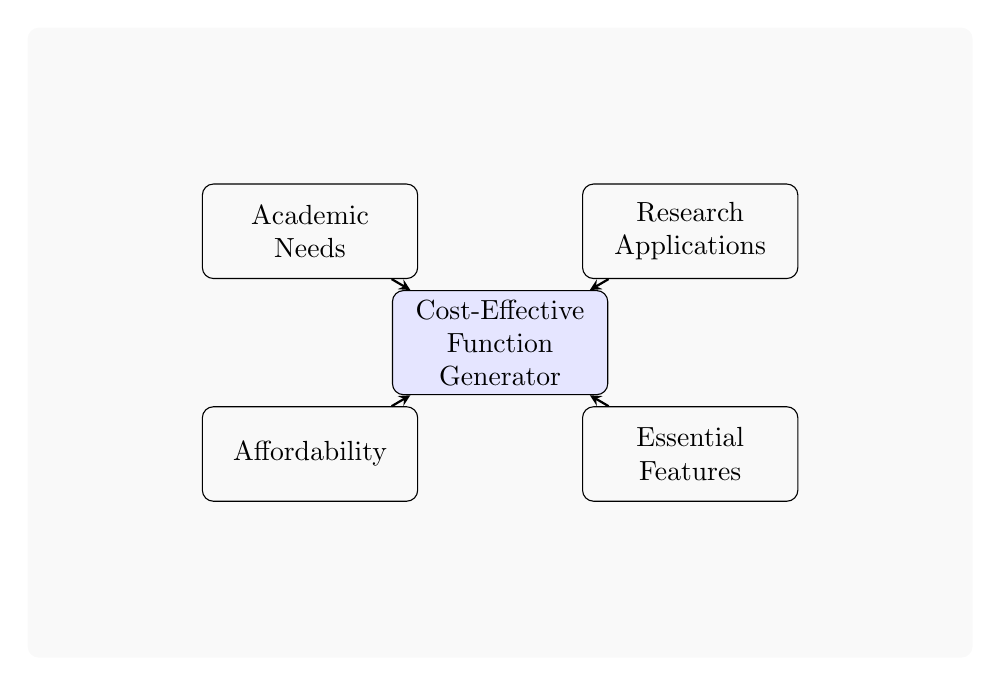
\begin{tikzpicture}[
    node distance = 2cm,
    block/.style = {rectangle, draw, rounded corners, minimum width=2.5cm, minimum height=1.2cm, text centered, text width=2.5cm},
    arrow/.style = {thick, ->, >=stealth}
]
    % Central motivation
    \node[block, fill=blue!10] (main) {Cost-Effective Function Generator};
    
    % Contributing factors (arranged in a circle)
    \node[block, above left of=main, xshift=-1cm] (academic) {Academic Needs};
    \node[block, above right of=main, xshift=1cm] (research) {Research Applications};
    \node[block, below left of=main, xshift=-1cm] (cost) {Affordability};
    \node[block, below right of=main, xshift=1cm] (features) {Essential Features};
    
    % Connecting arrows
    \draw[arrow] (academic) -- (main);
    \draw[arrow] (research) -- (main);
    \draw[arrow] (cost) -- (main);
    \draw[arrow] (features) -- (main);
    
    %background shading
    \begin{scope}[on background layer]
        \node[fill=gray!5, rounded corners, minimum width=12cm, minimum height=8cm] at (main) {};
    \end{scope}
\end{tikzpicture}

    \caption{Factors Driving the Function Generator Development}
    \label{fig:motivation}
\end{figure}

% Section: Requirements

\newpage
\section{Requirements}

\subsection{Input Requirements}
\begin{itemize}
    \item \textbf{Waveform Control:}
    \begin{itemize}
        \item System must accept digital inputs for waveform selection (Sine, Square, Triangle, Ramp, and Pulse waves)
    \end{itemize}
    \item \textbf{Frequency Range:}
    \begin{itemize}
        \item User input for frequency selection from 1Hz to 10MHz through rotary encoder interface
    \end{itemize}
    \item \textbf{Amplitude Control:}
    \begin{itemize}
        \item Variable amplitude control from 0V to 5V peak-to-peak through user interface
    \end{itemize}
    \item \textbf{Phase Control:}
    \begin{itemize}
        \item 0-360 degrees phase adjustment capability when needed
    \end{itemize}
    \item \textbf{Power Input:}
    \begin{itemize}
        \item Since, the client hasn’t specified the power requirements. We assume the power supply must be standard power supply, which can be usually available at laboratory spaces
    \end{itemize}
    \item \textbf{User Interface:}
    \begin{itemize}
        \item Rotary encoder with push-button functionality for parameter selection and adjustment, and buttons for user selection
    \end{itemize}
    \item \textbf{Digital Control:}
    \begin{itemize}
        \item SPI interface between ESP32 and AD9833 for waveform generation
    \end{itemize}
\end{itemize}

\subsection{Output Requirements}
\begin{itemize}
    \item \textbf{Waveform Quality:}
    \begin{itemize}
        \item Clean output waveforms with minimal distortion (THD < 1\% for sine wave)
    \end{itemize}
    \item \textbf{Frequency Accuracy: }
    \begin{itemize}
        \item Generated frequency must be as close to the desired value as possible
    \end{itemize}
    \item \textbf{Amplitude Stability:}
    \begin{itemize}
        \item Output amplitude must remain stable as close as possible to the desired value
    \end{itemize}
    \item \textbf{Display Output:}
    \begin{itemize}
        \item Real-time display of frequency, waveform type, and amplitude settings on OLED/LCD
    \end{itemize}
    \item \textbf{Signal Output:}
    \begin{itemize}
        \item Industry-standard BNC connector with 50\(\Omega\) output impedance
    \end{itemize}
    \item \textbf{Noise Level:}
    \begin{itemize}
        \item Output signal-to-noise ratio to be kept as high as possible
    \end{itemize}
\end{itemize}

\subsection{Power Requirements}
\begin{itemize}
    \item \textbf{Input Power Source:}
    \begin{itemize}
        \item USB Type-C power delivery
        \item Standard mobile charger (5V)
        \item Power rating: 15W-20W capability recommended
    \end{itemize}
    \item \textbf{Protection:}
    \begin{itemize}
        \item Over-current protection for >2.5A
        \item Reverse polarity protection
        \item Short circuit protection
        \item Thermal protection
    \end{itemize}
    \item \textbf{Power Supply Requirements:}
    \begin{itemize}
        \item USB Type-C charger: 5V/3A or better
        \item Good quality power supply recommended
    \end{itemize}
\end{itemize}

\subsection{Environmental Requirements}
\begin{itemize}
    \item \textbf{Operating Conditions:}
    \begin{itemize}
        \item Temperature: +0°C to +40°C.
        \item Humidity: Up to 80\% relative humidity (non-condensing).
    \end{itemize}
    \item \textbf{Storage Conditions:}
    \begin{itemize}
        \item Temperature: -10°C to +70°C.
        \item Humidity: Up to 70\% relative humidity.
    \end{itemize}
\end{itemize}

\subsection{Site (Usage Site) Requirements}
\begin{itemize}
    \item \textbf{Location:}
    \begin{itemize}
        \item Designed for indoor use in laboratory or workshop environments.
    \end{itemize}
    \item \textbf{Space Requirements:}
    \begin{itemize}
        \item Compact design to fit on standard lab benches (dimensions: 20cm x 15cm x 5cm maximum).
    \end{itemize}
    \item \textbf{Power Supply:}
    \begin{itemize}
        \item Standard 5V power source availability.
    \end{itemize}
    \item \textbf{Ventilation:}
    \begin{itemize}
        \item Adequate airflow around the device to prevent overheating.
    \end{itemize}
    \item \textbf{Lighting:}
    \begin{itemize}
        \item Sufficient lighting for display readability.
    \end{itemize}
\end{itemize}

\subsection{Structural Requirements}
\begin{itemize}
    \item \textbf{Dimensions:}
    \begin{itemize}
        \item Maximum size of 200mm × 150mm × 100mm.
    \end{itemize}
    \item \textbf{Material:}
    \begin{itemize}
        \item \textbf{Enclosure:} 2mm aluminium sheets for durability and heat dissipation or some enclosure which provides shielding.
        \item \textbf{Front Panel:} 2mm acrylic sheet for labeling and controls.
    \end{itemize}
    \item \textbf{Components:}
    \begin{itemize}
        \item Rotary encoders, rotary potentiometer, BNC connectors, push buttons, square push button.
    \end{itemize}
    \item \textbf{Assembly:}
    \begin{itemize}
        \item Modular design for easy assembly and disassembly.
        \item Rubber stoppers for stability and vibration damping.
        \item Bolts and nuts for secure fastening.
    \end{itemize}
    \item \textbf{Slidable Top Lid:}
    \begin{itemize}
        \item For easy access to internal components during maintenance.
    \end{itemize}
    \item \textbf{Access Points:}
    \begin{itemize}
        \item Easy access to calibration and test points.
    \end{itemize}
\end{itemize}

\subsection{Time Requirements}
\begin{itemize}
    \item \textbf{Design Time Requirement:}
    \begin{itemize}
        \item Total design time: 4 weeks
        \item Week 1: Ideation and concept development
        \item Weeks 2-4: Design implementation and testing
        \begin{itemize}
            \item Week 1: Simulations and parameter identification
            \item Week 2: Basic assembly and initial testing
            \item Week 3: Detailed testing and refinement
        \end{itemize}
    \end{itemize}
    \item \textbf{Time to Market Requirement:}
    \begin{itemize}
        \item Prototype completion: 4 weeks from project initiation
        \item First unit delivery: End of week 4
        \item Total time to market: 4 weeks
    \end{itemize}
    \item \textbf{Lifetime Requirement:}
    \begin{itemize}
        \item Minimum operational lifetime: 2 years
        \item Maintenance interval: Every 6 months
        \item Component lifetime specifications:
        \begin{itemize}
            \item Electronic components: Minimum 2 years
            \item Mechanical components: 10,000 operations
            \item Display: 10,000 hours
        \end{itemize}
        \item Performance degradation limits:
        \begin{itemize}
            \item Frequency drift: $\pm$1\% per year
            \item Amplitude drift: $\pm$2\% per year
        \end{itemize}
    \end{itemize}
    \item \textbf{End of Life Requirement:}
    \begin{itemize}
        \item Disposal requirements:
        \begin{itemize}
            \item Electronic components: Separate for e-waste disposal
            \item Material segregation: Separate plastic and metal components
        \end{itemize}
        \item Recycling specifications:
        \begin{itemize}
            \item Metal case: 100\% recyclable
            \item PCB: E-waste recycling protocol
            \item Components: Material-type separation required
        \end{itemize}
        \item Post-production support:
        \begin{itemize}
            \item Spare parts availability: 1 year after end-of-life
            \item Support timeline: 3 years after end-of-life
        \end{itemize}
    \end{itemize}
\end{itemize}


% % Section 3: Design and Methodology
% \section{Design and Methodology}
% \subsection{Requirements}
% Following is the list the technical and non-technical requirements of the function generator.
% \subsubsection{Input Requirements}
% \begin{itemize}
%     \item \textbf{Waveform Control:}
%     \begin{itemize}
%         \item System must accept digital inputs for waveform selection (Sine, Square, Triangle, Ramp, and Pulse waves)
%     \end{itemize}
%     \item \textbf{Frequency Range:}
%     \begin{itemize}
%         \item User input for frequency selection from 1Hz to 10MHz through rotary encoder interface
%     \end{itemize}
%     \item \textbf{Amplitude Control:}
%     \begin{itemize}
%         \item Variable amplitude control from 0V to 5V peak-to-peak through user interface
%     \end{itemize}
%     \item \textbf{Phase Control:}
%     \begin{itemize}
%         \item 0-360 degrees phase adjustment capability when needed
%     \end{itemize}
%     \item \textbf{Power Input:}
%     \begin{itemize}
%         \item Since, the client hasn’t specified the power requirements. We assume the power supply must be standard power supply, which can be usually available at laboratory spaces
%     \end{itemize}
%     \item \textbf{User Interface:}
%     \begin{itemize}
%         \item Rotary encoder with push-button functionality for parameter selection and adjustment, and buttons for user selection
%     \end{itemize}
%     \item \textbf{Digital Control:}
%     \begin{itemize}
%         \item SPI interface between ESP32 and AD9833 for waveform generation
%     \end{itemize}
% \end{itemize}

% \begin{figure}[H]
%     \centering
%     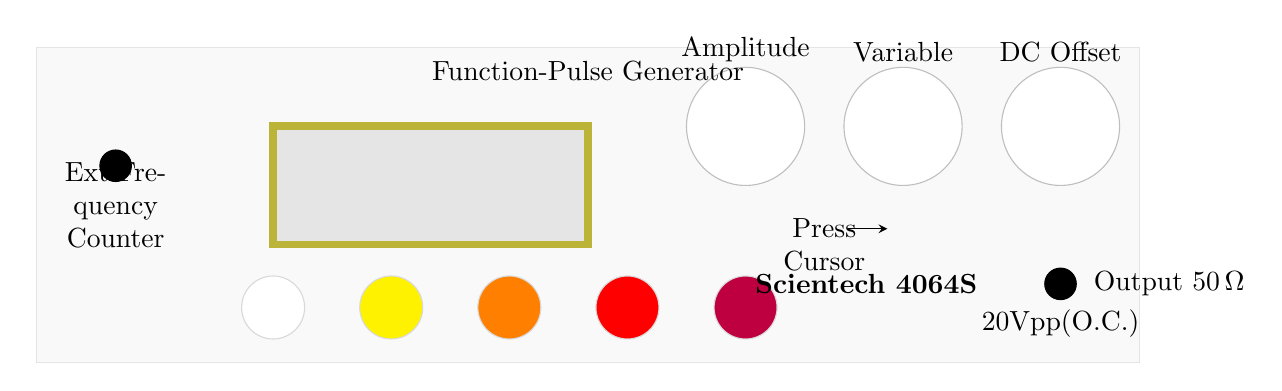
\begin{tikzpicture}[
    knob/.style={circle, draw=gray!50, fill=white, minimum size=15mm},
    button/.style={circle, draw=gray!30, fill=#1, minimum size=8mm},
    port/.style={circle, draw=black, fill=black, minimum size=4mm}
]
    % Main panel background
    \fill[gray!5] (0,0) rectangle (14,4);
    \draw[gray!20] (0,0) rectangle (14,4);
    
    % LCD Display
    \fill[black!10] (3,1.5) rectangle (7,3);
    \draw[yellow!70!black, line width=1mm] (3,1.5) rectangle (7,3);
    
    % Left port (Counter)
    \node[port] at (1,2.5) {};
    \node[text width=2cm, align=center] at (1,2) {Ext Frequency\\Counter};
    
    % Knobs on right side
    \node[knob] (amp) at (9,3) {};
    \node[above] at (9,3.7) {Amplitude};
    
    \node[knob] (var) at (11,3) {};
    \node[above] at (11,3.7) {Variable};
    
    \node[knob] (dc) at (13,3) {};
    \node[above] at (13,3.7) {DC Offset};
    
    % Output port
    \node[port] at (13,1) {};
    \node[right] at (13.3,1) {Output \SI{50}{\ohm}};
    \node[text width=2cm, align=center] at (13,0.5) {20Vpp(O.C.)};
    
    % Control buttons
    \node[button=white] at (3,0.7) {};
    \node[button=yellow] at (4.5,0.7) {};
    \node[button=orange] at (6,0.7) {};
    \node[button=red] at (7.5,0.7) {};
    \node[button=purple] at (9,0.7) {};
    
    % Title text
    \node[align=center] at (7,3.7) {Function-Pulse Generator};
    
    % Brand name
    \node[right] at (9,1) {\textbf{Scientech 4064S}};
    
    % Small cursor icon
    \path (10,1.5) node[align=center] {Press\\Cursor};
    \draw[->,>=stealth] (10.3,1.7) -- (10.8,1.7);
\end{tikzpicture}
%     \caption{User-supplied input on the front panel}
%     \label{fig:front_pabel}
% \end{figure}
% \subsubsection{Output Requirements}
% \begin{itemize}
%     \item \textbf{Waveform Quality:}
%     \begin{itemize}
%         \item Clean output waveforms with minimal distortion (THD < 1\% for sine wave)
%     \end{itemize}
%     \item \textbf{Frequency Accuracy: }
%     \begin{itemize}
%         \item Generated frequency must be as close to the desired value as possible
%     \end{itemize}
%     \item \textbf{Amplitude Stability:}
%     \begin{itemize}
%         \item Output amplitude must remain stable as close as possible to the desired value
%     \end{itemize}
%     \item \textbf{Display Output:}
%     \begin{itemize}
%         \item Real-time display of frequency, waveform type, and amplitude settings on OLED/LCD
%     \end{itemize}
%     \item \textbf{Signal Output:}
%     \begin{itemize}
%         \item Industry-standard BNC connector with 50\(\Omega\) output impedance
%     \end{itemize}
%     \item \textbf{Noise Level:}
%     \begin{itemize}
%         \item Output signal-to-noise ratio to be kept as high as possible
%     \end{itemize}
% \end{itemize}
% \subsubsection{Power Requirements}
% \begin{itemize}
%     \item \textbf{Input Power Source:}
%     \begin{itemize}
%         \item USB Type-C power delivery
%         \item Standard mobile charger (5V)
%         \item Power rating: 15W-20W capability recommended

%     \end{itemize}
%     \item \textbf{Protection:}
%     \begin{itemize}
%         \item Over-current protection for >2.5A
%         \item Reverse polarity protection
%         \item Short circuit protection
%         \item Thermal protection

%     \end{itemize}
    
%     \item \textbf{Power Supply Requirements:}
%     \begin{itemize}
%         \item USB Type-C charger: 5V/3A or better
%         \item Good quality power supply recommended
%     \end{itemize}
% \end{itemize}
    
% \subsubsection{Environmental Requirements}
% \begin{itemize}
%     \item \textbf{Operating Conditions:}
%     \begin{itemize}
%         \item Temperature: +0°C to +40°C.
%         \item Humidity: Up to 80\% relative humidity (non-condensing).
%     \end{itemize}
%     \item \textbf{Storage Conditions:}
%     \begin{itemize}
%         \item Temperature: -10°C to +70°C.
%         \item Humidity: Up to 70\% relative humidity.
%     \end{itemize}
% \end{itemize}
% \subsubsection{Site (Usage Site) Requirements}
% \begin{itemize}
%     \item \textbf{Location:}
%     \begin{itemize}
%         \item Designed for indoor use in laboratory or workshop environments.
%     \end{itemize}
%     \item \textbf{Space Requirements:}
%     \begin{itemize}
%         \item Compact design to fit on standard lab benches (dimensions: 20cm x 15cm x 5cm maximum).
%     \end{itemize}
%     \item \textbf{Power Supply:}
%     \begin{itemize}
%         \item Standard 5V power source availability.
%     \end{itemize}
%     \item \textbf{Ventilation:}
%     \begin{itemize}
%         \item Adequate airflow around the device to prevent overheating.
%     \end{itemize}
%     \item \textbf{Lighting:}
%     \begin{itemize}
%         \item Sufficient lighting for display readability.
%     \end{itemize}
% \end{itemize}

% \subsubsection{Structural Requirements}
% \begin{itemize}
%     \item \textbf{Dimensions:}
%     \begin{itemize}
%         \item Maximum size of 200mm × 150mm × 100mm.
%     \end{itemize}
%     \item \textbf{Material:}
%     \begin{itemize}
%         \item \textbf{Enclosure:} 2mm aluminium sheets for durability and heat dissipation or some enclosure which provides shielding.
%         \item \textbf{Front Panel:} 2mm acrylic sheet for labeling and controls.
%     \end{itemize}
%     \item \textbf{Components:}
%     \begin{itemize}
%         \item Rotary encoders (qty=2), rotary potentiometer (qty=1), BNC connectors (qty=1), push buttons (qty=5), square push button (qty=1).
%     \end{itemize}
%     \item \textbf{Assembly:}
%     \begin{itemize}
%         \item Modular design for easy assembly and disassembly.
%         \item Rubber stoppers (qty=4) for stability and vibration damping.
%         \item Bolts and nuts (qty=15 pairs) for secure fastening.
%     \end{itemize}
%     \item \textbf{Slidable Top Lid:}
%     \begin{itemize}
%         \item For easy access to internal components during maintenance.
%     \end{itemize}
%     \item \textbf{Access Points:}
%     \begin{itemize}
%         \item Easy access to calibration and test points.
%     \end{itemize}
% \end{itemize}

% \subsubsection{Time Requirements}
% \begin{itemize}
%     \item \textbf{Design Time Requirement:}
%     \begin{itemize}
%         \item Total design time: 4 weeks
%         \item Week 1: Ideation and concept development
%         \item Weeks 2-4: Design implementation and testing
%         \begin{itemize}
%             \item Week 1: Simulations and parameter identification
%             \item Week 2: Basic assembly and initial testing
%             \item Week 3: Detailed testing and refinement
%         \end{itemize}
%     \end{itemize}
%     \item \textbf{Time to Market Requirement:}
%     \begin{itemize}
%         \item Prototype completion: 4 weeks from project initiation
%         \item First unit delivery: End of week 4
%         \item Total time to market: 4 weeks
%     \end{itemize}
%     \item \textbf{Lifetime Requirement:}
%     \begin{itemize}
%         \item Minimum operational lifetime: 2 years
%         \item Maintenance interval: Every 6 months
%         \item Component lifetime specifications:
%         \begin{itemize}
%             \item Electronic components: Minimum 2 years
%             \item Mechanical components: 10,000 operations
%             \item Display: 10,000 hours
%         \end{itemize}
%         \item Performance degradation limits:
%         \begin{itemize}
%             \item Frequency drift: $\pm$1\% per year
%             \item Amplitude drift: $\pm$2\% per year
%         \end{itemize}
%     \end{itemize}
%     \item \textbf{End of Life Requirement:}
%     \begin{itemize}
%         \item Disposal requirements:
%         \begin{itemize}
%             \item Electronic components: Separate for e-waste disposal
%             \item Material segregation: Separate plastic and metal components
%         \end{itemize}
%         \item Recycling specifications:
%         \begin{itemize}
%             \item Metal case: 100\% recyclable
%             \item PCB: E-waste recycling protocol
%             \item Components: Material-type separation required
%         \end{itemize}
%         \item Post-production support:
%         \begin{itemize}
%             \item Spare parts availability: 1 year after final production
%             \item Upgrade path provided
%             \item Alternative product recommendations available
%         \end{itemize}
%     \end{itemize}
% \end{itemize}

% \subsubsection{Other Non-Functional Requirements
% }
% \begin{itemize}
%     \item \textbf{Color:}
%     \begin{itemize}
%         \item Grey for a professional appearance.
%     \end{itemize}
%     \item \textbf{Weight:}
%     \begin{itemize}
%         \item Approximately 1 kg for portability.
%     \end{itemize}
%     \item \textbf{Safety:}
%     \begin{itemize}
%         \item Proper insulation to prevent electrical hazards
%         \item No exposed wires or sharp edges.
%         \item Grounded chassis for shock protection.
%     \end{itemize}
%     \item \textbf{Serviceability:}
%     \begin{itemize}
%         \item Modular design for easy repair and component replacement.
%         \item Slidable top lid for quick access to internal parts.
%     \end{itemize}
%     \item \textbf{Reliability:}
%     \begin{itemize}
%         \item Stable performance under specific environmental conditions.
%     \end{itemize}
% \end{itemize}

% Section 5: Discussion
\section{Discussion}
Discuss the results and their implications. Highlight any challenges faced and how they were addressed. Suggest potential improvements or future work.



% Section 6: Who is the Single Point of Contact (SPOC)?




% Section 10: References
\section{References}
Use Zotero or another reference manager to format citations in APA/IEEE/MLA style:
\begin{thebibliography}{99}
    \bibitem{example} Author Name, \textit{Title of Reference}, Publisher, Year.
\end{thebibliography}

% Section 11: Appendices
\appendix
\section{Appendices}
\subsection{Appendix A: Circuit Diagrams}
Additional circuit diagrams.

\subsection{Appendix B: Code}
Include any code used for generating waveforms or analyzing data.

\end{document}
